\documentclass[a4paper]{scrartcl}

\usepackage{balance}  % to better equalize the last page
\usepackage{graphicx} % for EPS, load graphicx instead
\usepackage{url}      % llt: nicely formatted URLs
\usepackage{amsmath}
\usepackage{mdframed}
\usepackage[table]{xcolor}
\usepackage{cite}
\usepackage{url}


\title{A symmetry breaking SAT encoding for the social golfer problem}
\author{Dennis Lewandowski \\
    RWTH Aachen University \\
    Seminar: Satisfiability Checking \\
    Matr. Nr. 317071
    }
\date{2014-07-11}

\begin{document}

\maketitle

\begin{abstract}

The increasing performance of modern SAT solvers encourages the reduction of problems from other areas, such as combinatorial problems, into SAT problems. To get the best performance, the encoding has to regard features of the problem, such as symmetry, as well as features of the solver. In this paper, we will present and analyze an encoding for the \emph{Social Golfer Problem}, a problem with a high degree of symmetry. We will add symmetry breaking constraints to the encoding and discuss how this effects the performance of different types of solvers. 

\end{abstract}

\section{Introduction}

A lot of effort has been put into developing faster and better SAT solvers in the recent years (\url{http://satcompetition.org/2014/}, \url{http://aclib.net/cssc2014/}). With solvers becoming more efficient, it becomes apparent to use SAT solving for problems where solvers are not as performant, or for which no solver is available. These problems include combinatorial problems or constraint problems.

Modeling a problem into SAT can lead to different inefficiencies. For example, a constraint problem that consists of only few constraints can grow into millions of clauses when encoded into SAT. The SAT encoding might lose important structural features of the problem, such as symmetry or linearity, which can greatly influence the performance of the used solver\cite{ramani}.

While a lot of research is done on optimizing SAT solvers, a great deal of optimization can be achieved using the right encoding for the problem. When choosing an encoding, there are trade-offs to be made between different aspects of the encoding. One could aim for an encoding that is intuitive and easily understandable. It could be desired to have a minimum set of variables, minimizing the space of possible variable assignments and therefore speeding up computation. It could take into account specific features of the problem, such as symmetries in combinatorial problems.

In the following, we will present an encoding for the \emph{Social Golfer Problem} as proposed by Gent et al.\cite{Gent05}. The encoding will use an intuitive set of variables that allows to state most constraints of the problem in easy readable clauses. It will also preserve the symmetrical nature of the problem. We will then try to eliminate these symmetries and examine the effects this measure has on the performance of different kinds of SAT solvers.

\subsection{The Social Golfer Problem}

The Social Golfer Problem is a famous combinatorial problem. The task is to find a schedule of play for a group of golfers that lasts as many weeks as possible. The constraints for this problem are:

\begin{mdframed}[skipabove=\baselineskip, skipbelow=\baselineskip, leftmargin=20, rightmargin=20]

\begin{enumerate}
    \item A golf club has 32 members.
    \item Each member plays golf once in a week.
    \item Golfers always play in groups of 4
    \item No golfer plays in the same group as any other golfer twice
\end{enumerate}

\end{mdframed}

The number of weeks, players and the size of groups are generalizable. The general problem is characterized a triple $(w,p,g)$, where $w$ is the number of weeks, $p$ is the number of players per group and $g$ is the number of groups playing. The general Social Golfer Problem represents a class of different combinatorial problems. One example of a concrete problem from this class of problems is \emph{Kirkman's Schoolgirl Problem}, given by the tuple $(7,3,5)$:

\begin{mdframed}[skipabove=\baselineskip, skipbelow=\baselineskip, leftmargin=20, rightmargin=20]

Fifteen young ladies in a school walk out three abreast for seven days in succession: it is required to arrange them daily so that no two shall walk twice abreast.

\end{mdframed}

A tuple of $(1,2,(n/2))$ represents the problem of constructing a round-robin schedule for a two-player tournament, where $n$ is the number of players. The Social Golfer Problem itself is described by the tuple $(w,4,8)$. The overall goal is to find a maximal value for $w$. With 32 players and each player facing 3 new other players each week, $w$ can not be greater than 10. Since a solution for a 9 weeks schedule has already been posted, we will concentrate on finding a solution for 10 weeks.

\subsection{Symmetries in Combinatorial Problems}

In many combinatorial it is necessary to group entities together by a given set of constraints. In these cases, the order of entities within such groups can be considered irrelevant. Sometimes even the order of groups is considered irrelevant. Whenever two solutions for a problem can be transformed into each other by exchanging entities within groups, these solutions are called \emph{symmetrical}. Symmetrical solutions build up equivalence classes which either contain only solutions or no solutions\cite{Smith01}.

In the following, we will present an excerpt of a solution for \emph{Kirkman's Schoolgirl Problem}, which we presented in the section before. The presented solution shows the assignment of schoolgirls, denoted by letters from \emph{A} to \emph{O}, into groups of three on two days of the week:

\begin{table}[h]
\centering
\begin{tabular}{ l | l  l  l l  l }
Day & Group 1 & Group 2 & Group 3 & Group 4 & Group 5 \\
\hline
Sunday & ABC & DEF & GHI & JKL & MNO \\
Monday & ADH  & BEK & CIO & FLN & GJM \\
\end{tabular}
\end{table}

Obviously, the solution stays valid if we change the order of schedules between days:

\begin{table}[h]
\centering
\begin{tabular}{ l | l  l  l l  l }
Day & Group 1 & Group 2 & Group 3 & Group 4 & Group 5 \\
\hline
\emph{Sunday} & ADH  & BEK & CIO & FLN & GJM \\
\emph{Monday} & ABC & DEF & GHI & JKL & MNO \\
\end{tabular}
\end{table}

We can even change the order of groups within every week:

\begin{table}[h]
\centering
\begin{tabular}{ l | l  l  l l  l }
Day & Group 1 & Group 2 & Group 3 & Group 4 & Group 5 \\
\hline
Sunday & \emph{DEF} & \emph{ABC} & GHI & JKL & MNO \\
Monday & ADH  & BEK & CIO & \emph{GJM} & \emph{FLN}\\
\end{tabular}
\end{table}

Symmetries within a solution space produce redundant search paths, which slow down backtracking search. When a partial assignment is proven to lead to an unsatisfying assignment, all symmetrical assignments will also lead to an unsatisfying assignment. This leads to the conclusion that a solver could work more efficient if these symmetrical assignments are ignored by the solver. Removing symmetries also reduces to solution space, which seems beneficial for solvers, as they do not have to make as many assignments compared to a solution space that contains symmetrical solutions.

\begin{figure}[h!]
\centering
    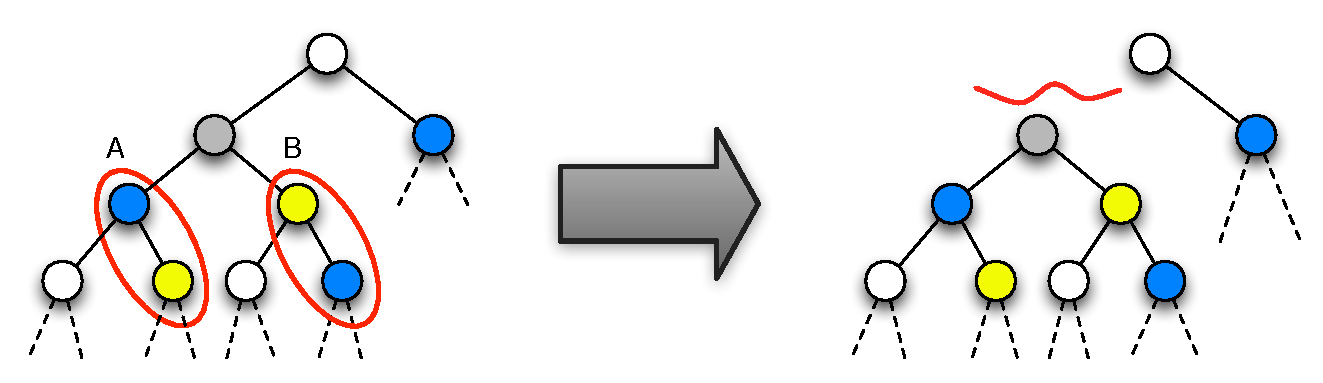
\includegraphics[width=13.6cm]{images/symmetry_breaking}
    \caption{An illustration of how symmetry breaking reduces the solution space: A and B present partial symmetrical assignments that are unsatisfying. Removing any following symmetrical assignments reduces the overall solution space.}
\end{figure}

Symmetries can be removed in the following ways:

\begin{enumerate}
\item \emph{Remodel} the problem
\item Add more \emph{constraints} to the model
\item \emph{Avoid} symmetrically equivalent states during search
\end{enumerate}

The goal of \emph{remodeling} the problem is achieving a model that has less inherent symmetries. For example, enumerating the instances or groups within a problem will yield a highly symmetrical solution space. This is because the entities and groups are modeled distinguishable. Modeling the problem without any symmetries often times leads to the use of highly abstract variables, which takes a lot of effort. The effort of finding a model with no symmetry can out score the extra time the solver would need to solve the problem using a model that has symmetries.

When \emph{adding symmetry breaking constraints} to the model, the original model of the problem stays the same. Additional constraints can produce computation overhead, which may in turn negate the effect of a smaller solution space. First-solution-search can be slowed down significantly, depending on the solver that is used\cite{Prestwich}.

In order to \emph{avoid symmetrical equivalent states during search}, the solver needs to be able to constantly check for the presence of symmetrical solutions before branching decisions. As this produces computation overhead, such a solver can no longer be efficient for solving problems with less to no symmetry. Therefore, this approach has not found success in SAT solving.

\section{Encoding of the Social Golfer Problem}

In this section we encode the constraints of the Social Golfer Problem. The first group of constraints deals with the number of groups a golfer can be assigned to, the number of weeks that a group can be assigned to, et cetera. We will refer to this as \emph{``external constraints''}, as they set the framework within which we can assign golfers to groups and groups to weeks.

The second group of constraints deals with the rule that each golfer is only allowed to play with each other player once. We will refer to this constraint as \emph{``internal constraint''}, as it deals with conflicts occurring in an assignment which is valid within the external constraints.


\subsection{Modeling external constraints}

In order to model the Social Golfer Problem, we first need to define a model that represents whether a certain golfer plays in a certain week within a certain group. In addition to this, our model will also state that a given golfer is at a certain position within a group. With respect to our ambition of eliminating symmetries within the model, this seems certainly contradictory, since introducing any kind of order into a set of exchangeable entities will introduce additional symmetries. However, this way of modeling allows to state most of the constraints as ``at-most-one'' and ``at-least-one'' clauses, making the constraints themselves more intuitive.

Let $x = p \times g$ be the number of players. The first variable introduced to our model is $\textsc{Golfer}_{ijkl}$, with $1 \leq i \leq x$, $1 \leq j \leq p$, $1 \leq k \leq g$ and $1 \leq l \leq w$.

The constraint that each golfer plays in at least one group every week is expressed in the following way:

\begin{equation}
\label{form:everyone_plays}
% Every golfer must play in every week in at least one group at at least one position
\centering
    \bigwedge \limits_{i=1}^x 
    \bigwedge \limits_{l=1}^w 
    \bigvee \limits_{j=1}^p
    \bigvee \limits_{k=1}^g 
    \textsc{Golfer}_{ijkl}
\end{equation}

To make sure that no golfer is assigned to more than on position inside a group, we'll add the following clauses:

\begin{equation}
% When a golfer plays at a position inside a group, he can not play on any other position in the same group
\centering
    \bigwedge \limits_{i=1}^x 
    \bigwedge \limits_{l=1}^w 
    \bigwedge \limits_{j=1}^p
    \bigwedge \limits_{k=1}^g 
    \bigwedge \limits_{m=j+1}^p 
    % \neg 
    \textsc{Golfer}_{ijkl} 
    \to
    % \vee 
    \neg \textsc{Golfer}_{imkl}
\end{equation}

The following clauses encode that no golfer plays in more than one group within the same week:

\begin{equation}
% When a golfer plays at a position inside a group within one week, he cannot play at any position and group in the same week
\centering
    \bigwedge \limits_{i=1}^x 
    \bigwedge \limits_{l=1}^w 
    \bigwedge \limits_{j=1}^p
    \bigwedge \limits_{k=1}^g 
    \bigwedge \limits_{m=k+1}^g 
    \bigwedge \limits_{n=j+1}^p 
    % \neg 
    \textsc{Golfer}_{ijkl} 
    \to
    % \vee 
    \neg \textsc{Golfer}_{inml}
\end{equation}

The next set of clauses ensures that every position in each group within each week is assigned to at least one golfer.

\begin{equation}
% On every day in every group at every position there is at least one golfer playing
\centering
    \bigwedge \limits_{l=1}^w 
    \bigwedge \limits_{k=1}^g 
    \bigwedge \limits_{j=1}^p
    \bigvee \limits_{i=1}^x 
    \textsc{Golfer}_{ijkl}
\end{equation}


Finally, the following set of clauses ensures that each position within each group is at most taken by one golfer.

\begin{equation}
% If within a week within a group a position is already taken by a golfer, this position can not be taken by another golfer
\centering
    \bigwedge \limits_{l=1}^w 
    \bigwedge \limits_{k=1}^g 
    \bigwedge \limits_{j=1}^p
    \bigwedge \limits_{i=1}^x 
    \bigwedge \limits_{m=i+1}^x 
    % \neg 
    \textsc{Golfer}_{ijkl} 
    \to
    % \vee 
    \neg \textsc{Golfer}_{imkl}
\end{equation}


\subsection{Modeling internal constraints}

The last constraint we need to add is the one that guarantees that no golfer plays in the same group as any other golfer twice. To ensure this, we will introduce a construction that is called a ``ladder matrix''.


\subsubsection{Constructing the ladder matrix}

\begin{table}[h]
\centering
\label{ladder:example}
\begin{tabular}{ l | l | l | l | l | l | l }

    & 1.1 & 1.2 & 2.1 & 2.2 & 3.1 & 3.2 \\
\hline
3.4 & --- & --- & --- & --- & --- & --- \\
2.3 & --- & --- & --- & --- & --- & --- \\
2.4 & --- & --- & --- & --- & --- & --- \\
1.2 & --- & --- & --- & --- & --- & --- \\
1.3 & --- & --- & --- & --- & --- & --- \\
1.4 & --- & --- & --- & --- & --- & --- \\

\end{tabular}
\caption{The ladder variables presented as a table for the Social Golfer Problem 3-2-2. Each row represents a unique combination of two players. Each column represents a group within a week.}
\end{table}

A ladder matrix is built with a set of auxiliary boolean ladder variables. The ladder variables will indicate whether two players are scheduled to play in a certain week within a certain group. We will denote the ladder variables as $\text{Ladder}_{yz}$, where $1 \leq y \leq {x \choose 2}$ and $1 \leq z \leq g \times w$. Values of $y$ indicate a match between two players, values of $z$ represent a combination of a week and a team number (see table \ref{ladder:example}). 



Because we constructed variables for exactly ${x \choose 2}$, we end up with a set of all combinations of weeks and groups for each unique pair of two players. The next thing we need to do is to make sure that once a pair of players is assigned into one group within one week, this pair is not assigned any other group in any other week.

Consider the ladder variables for a fixed pair of players. We define such a row to be valid if and only if it is built of a sequence of zero or more \textsc{true} assignments, followed only by \textsc{false} assignments. So once a ladder variable within a row is set to \textsc{false}, each subsequent variable must also be \textsc{false}. This is achieved by adding clause \ref{ladder:propagation}:

\begin{equation}
\label{ladder:propagation}
\centering
    \bigwedge \limits_{y=1}^{{x \choose 2}}
    \bigwedge \limits_{z=1}^{(g \times w)-1}
    \text{Ladder}_{yz+1}
    \to
    \text{Ladder}_{yz}
\end{equation}

Given this encoding, we define that a pair of players is assigned a group $k$ and a week $l$ when the ladder variable in their respective row is \textsc{false} for the first time. As an example consider the following assignment of ladder variables for the match between the players 1 and 2:

\begin{table}[h]
\centering
\begin{tabular}{ l | l | l | l | l | l | l }
    & 1.1 & 1.2 & 2.1 & 2.2 & 3.1 & 3.2 \\
\hline
1.2 & T & T & \textbf{T} & \textbf{F} & F & F \\
\end{tabular}
\end{table}

With respect to \ref{ladder:propagation} this is a valid assignment of ladder variables. The change from \textsc{true} assignments to \textsc{false} assignments from column 2.1 to column 2.2 (emphasized in bold) schedules player 1 and 2 to play within group 1 in week 2. Because of \ref{ladder:propagation} it is no longer possible to schedule this pair of players to another group in another week. So no golfer can play with another golfer in the same group more than once.


\subsection{Matching entries of the ladder matrix to the $\textsc{Golfer}$ variable}

Finally we need to link the results of the assignment of our ladder matrix to our set of external constraints. First, we introduce an auxiliary variable $\textsc{Golfer'}_{ikl}$, with $1 \leq i \leq x$, $1 \leq k \leq g$ and $1 \leq l \leq w$. This variable is assigned \textsc{true}, when the golfer $i$ is scheduled to play in group $k$ in week $l$. The relation to the $\textsc{Golfer}_{ijkl}$ in the external constraints is established with the following set of clauses:

\begin{equation}
    \textsc{Golfer'}_{ikl} \iff \bigvee \limits_{j=1}^p \textsc{Golfer}_{ijkl}
\end{equation}

We will then relate the $\textsc{Golfer'}_{ikl}$ variable to the ladder matrix in such a way, that no golfer plays in the same group as any other golfer more than once. Whenever $\textsc{Golfer'}_{ikl}$ and $\textsc{Golfer'}_{mkl}$ for some golfers $m$ and $i$ are satisfied, both golfers play in the same group $k$ at the same week $l$. In the ladder matrix, this is indicated by an assignment of \textsc{true} to the entry in the column with the index $i.k$ and the row with the index $i.m$ and an assignment of \textsc{false} of the entry in the next column of the same row. This is done by adding the following group of clauses:

\begin{equation}
\centering
    \bigwedge \limits_{l=1}^{w}
    \bigwedge \limits_{k=1}^{g}
    \bigwedge \limits_{i=1}^{x-1}
    \bigwedge \limits_{m=i+1}^{x}
    (\textsc{Golfer'}_{ikl} \wedge \textsc{Golfer'}_{mkl}) \to \text{Ladder}_{[{x-1 \choose 2}+m-i](l \times k)}
\end{equation}

\begin{equation}
\centering
    \bigwedge \limits_{l=1}^{w}
    \bigwedge \limits_{k=1}^{g}
    \bigwedge \limits_{i=1}^{x-1}
    \bigwedge \limits_{m=i+1}^{x}
    (\textsc{Golfer'}_{ikl} \wedge \textsc{Golfer'}_{mkl}) \to \neg \text{Ladder}_{[{x-1 \choose 2}+m-i](l \times k + 1)}
\end{equation}

Conversely, whenever the entries of a row for a match of two players change from \textsc{true} to \textsc{false}, the auxiliary \textsc{Golfer'} variables for the corresponding golfers need to be set to \textsc{true} accordingly. This can be achieved by adding the following clauses:

\begin{equation}
\centering
    \bigwedge \limits_{l=1}^{w}
    \bigwedge \limits_{k=1}^{g}
    \bigwedge \limits_{i=1}^{x-1}
    \bigwedge \limits_{m=i+1}^{x}
    \Big(
        \text{Ladder}_{
            [
                {x-1 \choose 2}
                +m-i
            ](l \times k)
        }
        \wedge
        \neg
        \text{Ladder}_{
            [
                {x-1 \choose 2}
                +m-i
            ](l \times k + 1)
        }
    \Big)
    \to
    \textsc{Golfer'}_{ikl}
\end{equation}

\begin{equation}
\centering
    \bigwedge \limits_{l=1}^{w}
    \bigwedge \limits_{k=1}^{g}
    \bigwedge \limits_{i=1}^{x-1}
    \bigwedge \limits_{m=i+1}^{x}
    \Big(
        \text{Ladder}_{
            [
                {x-1 \choose 2}
                +m-i
            ](l \times k)
        }
        \wedge
        \neg
        \text{Ladder}_{
            [
                {x-1 \choose 2}
                +m-i
            ](l \times k + 1)
        }
    \Big)
    \to
    \textsc{Golfer'}_{mkl}
\end{equation}

\section{Symmetry breaking}

As already mentioned when defining the \textsc{Golfer} variable, our model turns out to be highly symmetrical. Besides ordering weeks, groups and players, we introduced more symmetries by ordering players within a group into certain positions. A model with minimal symmetries would have to model players, weeks, groups and positions within as completely interchangeable. However, finding such an encoding might cost more effort than it could be counterbalanced with an efficient non-symmetrical encoding. 

In order to break the symmetry introduced through our encoding, we will add some symmetry-breaking clauses to the encoding. The main idea here is to force entities into a lexicographical order. First, we will enforce an increasing numerical order onto players within the same group, by prohibiting assignments where players with indices smaller than the player at a certain position are placed at positions with a higher index than the latter:

\begin{equation}
\centering
    \bigwedge \limits_{i=1}^x
    \bigwedge \limits_{j=1}^p
    \bigwedge \limits_{k=1}^g
    \bigwedge \limits_{l=1}^w
    \bigwedge \limits_{m=1}^{i-1}
    \textsc{Golfer}_{ijkl}
    \to
    \neg \textsc{Golfer}_{m(j+1)kl}
\end{equation}

More symmetries can be broken by forcing the first players of each group within one week into a lexicographical order. This is achieved by setting golfer number 1 as the first golfer in the first group within every week. Further we disallow assignments where golfers with a smaller index than the first golfer within a group are assigned the first golfer in a group with a bigger index than the latter:

\begin{equation}
\centering
    \bigwedge \limits_{i=1}^x
    \bigwedge \limits_{k=1}^g
    \bigwedge \limits_{l=1}^w
    \bigwedge \limits_{m=1}^{i-1}
    \textsc{Golfer}_{i1kl}
    \to
    \neg \textsc{Golfer}_{m1(k+1)l}
\end{equation}

Lastly we will break symmetries between weeks. For this, we enforce a lexicographical order onto the second players within each group between weeks in a manner similar to the ones before:

\begin{equation}
\centering
    \bigwedge \limits_{i=1}^x
    \bigwedge \limits_{k=1}^g
    \bigwedge \limits_{l=1}^w
    \bigwedge \limits_{m=1}^{i-1}
    \textsc{Golfer}_{i2kl}
    \to
    \neg \textsc{Golfer}_{m2k(l+1)}
\end{equation}


\section{Performance}

The goal of introducing symmetry breaking clauses was to speed up the solution finding process by reducing the search space through the elimination of redundant search paths. However, eliminating symmetries by adding symmetry breaking clauses, as presented in the previous section, also increases the number of clauses that need to be evaluated on every assignment. How does this influence the overall performance of a SAT solver?


\subsection{Performance Impact on Local Search}

For experimental evaluation of the presented encoding, Gent et al. used two different SAT solvers. The solvers are instance of the two classes of SAT solvers that are usually used in practice: Walksat\cite{walksat2004}, a local search solver, and Siege\cite{Ryan04}, a DPLL backtracking-based solver.

Walksat works by starting with an assigning random truth values to the variables of the model. From this assignment on it tries to find a better assignment by randomly flipping the truth assignments of variables in unsatisfied clauses. This is done until a satisfying assignment is found.

When used on satisfiable instances of the problem, Walksat was found to perform significantly slower when using the symmetry breaking model as compared to the model with symmetries. This conforms to the findings of Prestwich\cite{Prestwich}. Prestwich's evaluation of the effect of symmetry breaking for different kinds of SAT solvers showed that symmetry breaking constraints slow down solution finding for local search algorithms and also hybrids of local search and backtracking algorithms. As an interpretation he suggests that, by reducing the solution space, the density of solutions is also reduced, which makes it harder for a local search algorithm to find any first solution. However, the reduced solution space in turn might speed up \emph{exhaustive search}, as there are less solutions overall. As another suggestion he mentions the idea to \emph{maximize} solution symmetries in order to increase the chance of hitting a random assignment that is close to any of the symmetrical solutions right from the beginning.


\subsection{Performance Impact on Backtracking}

The other solver, Siege, is a modified version of the DPLL algorithm\cite{DPLL}. Siege uses randomized backtracking search and clause learning. As with Walksat, the symmetry breaking model does not perform as well as the model without symmetry breaking. This is contrary to Prestwich, who reported the effects of symmetry breaking on backtracking solvers to be ``strongly positive''\cite{Prestwich}. This again holds only for first-solution search, not for exhaustive search.


\section{Conclusion}

In this paper we explored an encoding for the Social Golfer Problem. As the problem was highly symmetrical, we took measures to remove these symmetries in the encoding. This was done by adding symmetry breaking constraints to the model. We then discussed the effects that symmetry breaking has on the performance of the different kinds of SAT solvers.

The presented encoding for the Social Golfer Problem used an intuitive variable set that allowed most constraints to be encoded into ``at least one'' and ``at most one'' clauses. The encoding introduced a lot of symmetries since it enumerated weeks, groups and golfers, and even added more symmetries by enumerating positions of golfers within teams. This enumerating led to an increased number of symmetry breaking clauses.

One of the main findings of the performance discussion is that the performance of a solver is depending on the encoding used for a problem and the kind of solution that is requested. For first solution search, on one hand symmetry breaking tends to have positive effects on the performance of backtracking algorithms, but strongly negative effects on local search algorithms. On the other hands, there are examples where the costs of added constraints for symmetry breaking does not pay back in solver performance, as it was with the encoding discussed in this paper.

A way to remove symmetries, without the additional costs of symmetry breaking clauses, would be to model the problem in a way that entities of problem are treated as interchangeably. However, it is often not possible to find a model which removes all symmetries.

Finally, the presented encoding made a trade-off between being understandable and being performant. It was tried to buy back performance that was lost in the encoding by adding symmetry breaking constraints. Adding these constraints did not pay of, but rather showed that the choice of an encoding can have a significant impact on the performance of the solver.

\bibliographystyle{acm}
\bibliography{social_golfer}

\end{document}